%Master File:lectures.tex

\lesson{Writing an Arrays}

\vspace*{-2cm}
\begin{center}
  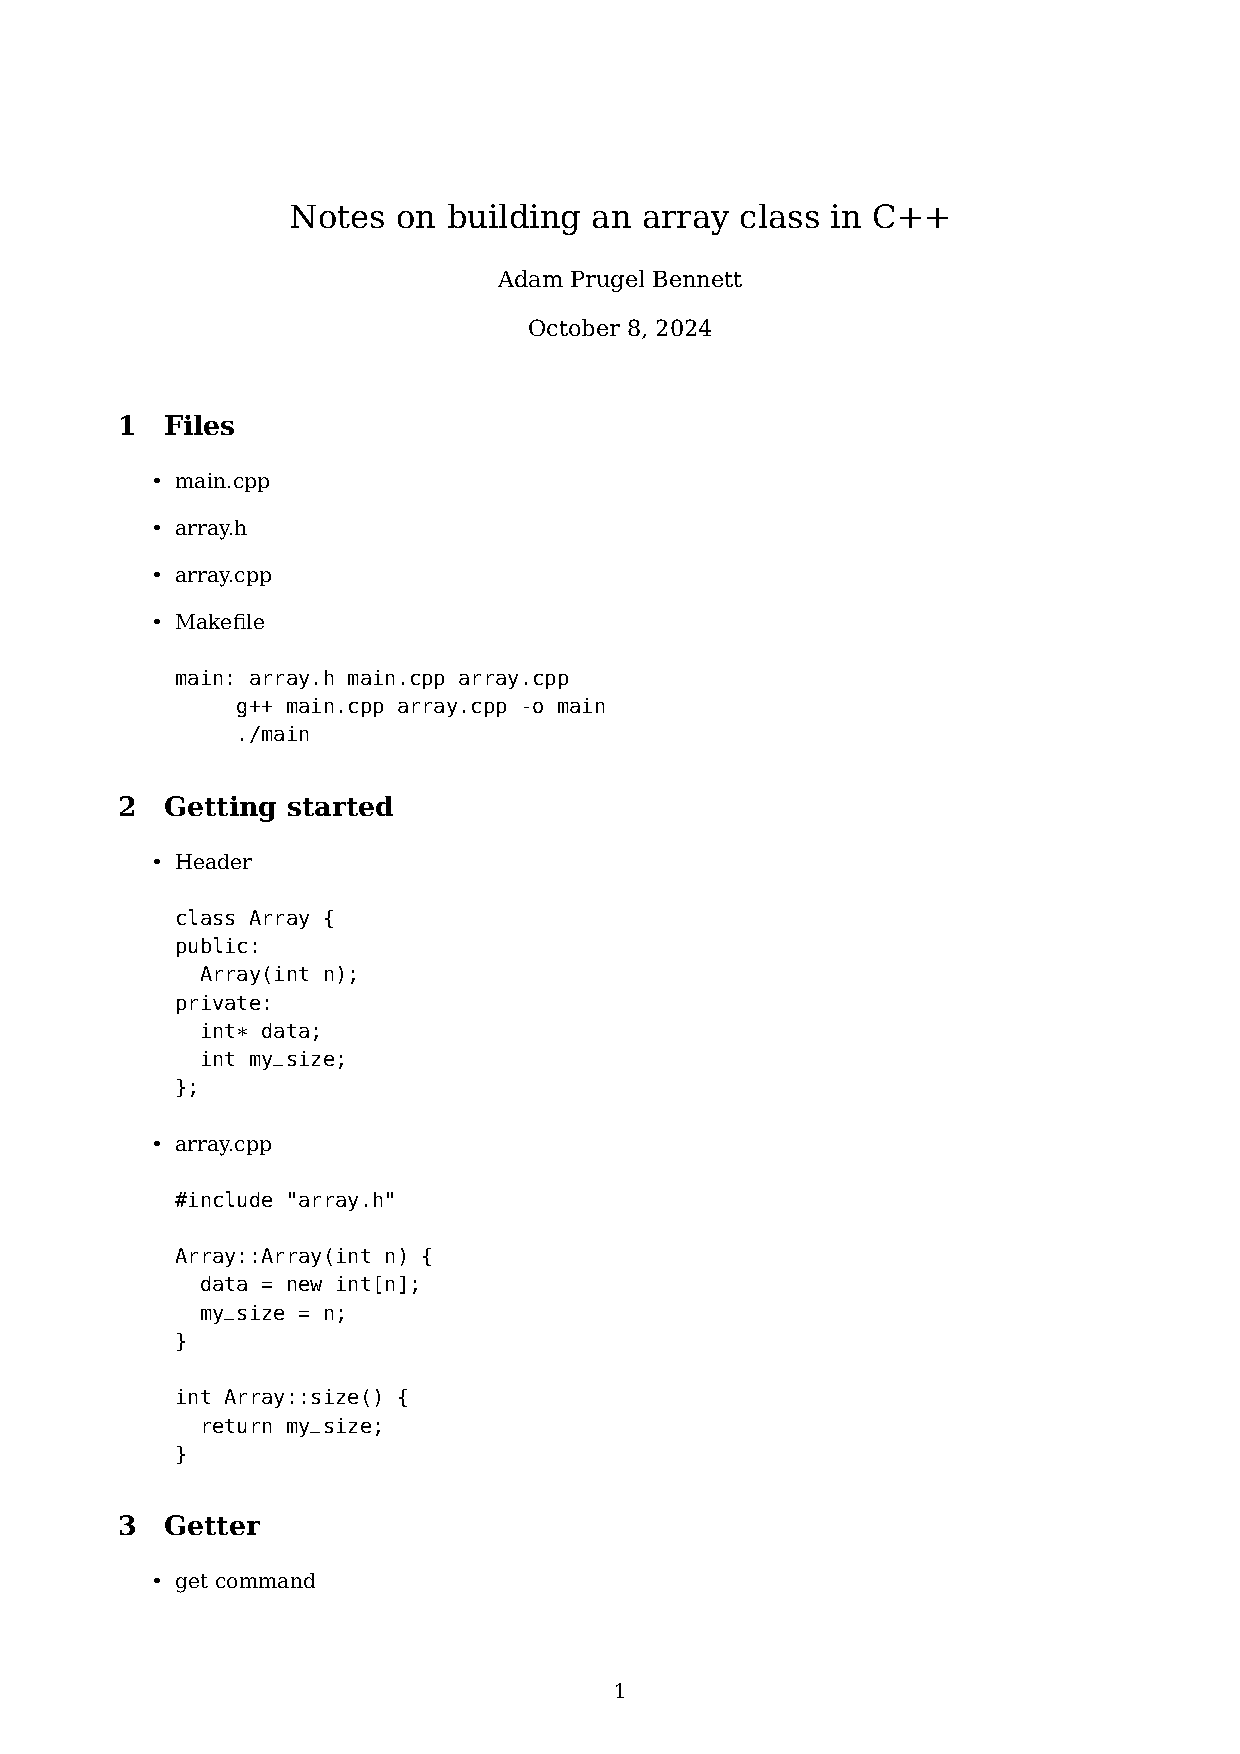
\includegraphics[height=11cm]{array}
\end{center}
\vspace*{-1cm}
\keywords{Writing data structures in C++}

%%%%%%%%%%%%%%%%%%%%%%% Next Slide %%%%%%%%%%%%%%%%%%%%%%%

\begin{slide}
  \section{This is not a lecture!}

  \begin{itemize}
  \item This is not being taught as a lecture, but run as a practical
    session
  \item We are going to write a resizable array class in C++
  \item I will call the class Array although this is not a great name
  \item The point of this is to understand the subtleties of coding is C++
  \end{itemize}

\end{slide}

%%%%%%%%%%%%%%%%%%%%%%% Next Slide %%%%%%%%%%%%%%%%%%%%%%%

\begin{slide}
  \section{Complied code}


  \begin{itemize}
  \item C++ like C must be compiled and linked
  \item Compiling turns the code into machine code (*.o files) with
    calls to external libraries
  \item Linking actually links the external libraries with the code to
    produce an executable file
  \item We use a \jl$Makefile$ to do the compile and linking
    \begin{cpp}
      all: main run

      main: array.h array.cc main.cc
          g++ main.cc array.cc -o main

      run: main
	  ./main

    \end{cpp}
  \end{itemize}

\end{slide}

%%%%%%%%%%%%%%%%%%%%%%% Next Slide %%%%%%%%%%%%%%%%%%%%%%%

\begin{slide}
\section{Cpp Style Classes: main.cc}

\begin{cpp}
#include <iostream>
#include "array.h"
using namespace std;

int main() {
  Array a(3);
  a.set(0,0);
  a.set(1,2);
  a.set(2,4);

  cout << a.get(0) << ", " << a.get(1) << ", " << a.get(2) << endl;

  return 0;
}
\end{cpp}
\end{slide}

%%%%%%%%%%%%%%%%%%%%%%% Next Slide %%%%%%%%%%%%%%%%%%%%%%%

\begin{slide}
\section{array.h}

\begin{cpp}
#ifndef ARRAY_H
#define ARRAY_H

class Array {
private:
  int *data;
public:
  Array(int n);
  void set(int index, int value);
  int get(int index);
};

#endif
\end{cpp}
\end{slide}

%%%%%%%%%%%%%%%%%%%%%%% Next Slide %%%%%%%%%%%%%%%%%%%%%%%

\begin{slide}
\section{array.cc}
\begin{cpp}
#include "array.h"

Array::Array(int n) {
  data = new int[n];
}

void Array::set(int index, int value) {
  data[index] = value;
}

int Array::get(int index) {
  return data[index];
}
\end{cpp}

\end{slide}

%%%%%%%%%%%%%%%%%%%%%%% Next Slide %%%%%%%%%%%%%%%%%%%%%%%

\begin{slide}
\section{Operator Overloading}

\begin{itemize}
\item Cpp is just ugly
\item C++ allows us to overload operators (e.g. \jl$+$, \jl$+=$,
  \jl$<<$, etc.)
\item One operator is indexing: \jl$operator[int]()$
\item We can use this to return a reference to \jl$data[i]$
  \begin{cpp}
int& Array::operator[](int index) {
  return data[index];
}
  \end{cpp}
\end{itemize}

\end{slide}

%%%%%%%%%%%%%%%%%%%%%%% Next Slide %%%%%%%%%%%%%%%%%%%%%%%

\begin{slide}
\section{Updated main.cc}
  
\begin{cpp}
#include <iostream>
#include "array.h"
using namespace std;

int main() {
  Array a(3);

  for(int i=0; i<3; i++) {
    a[i] = i*i;
  }

  cout << a[0] << ", " << a[1] << ", " << a[2] << endl;

  return 0;
}
\end{cpp}
\end{slide}

%%%%%%%%%%%%%%%%%%%%%%% Next Slide %%%%%%%%%%%%%%%%%%%%%%%

\begin{slide}
  \section[-2]{Adding Power}
  
  \begin{itemize}
  \item As we might want to print different arrays lets create a print
    function
  \item We want Array to know how many elements are in it
    \begin{cpp}
#ifndef ARRAY_H
#define ARRAY_H

class Array {
private:
  int *data;
  int length;
public:
  Array(int n);
  int& operator[](int index);
  int size();
};

#endif
    \end{cpp}
  \end{itemize}


\end{slide}

%%%%%%%%%%%%%%%%%%%%%%% Next Slide %%%%%%%%%%%%%%%%%%%%%%%

\begin{slide}
\section[-2]{main.cc}

\begin{cpp}
#include <iostream>
#include "array.h"
using namespace std;

void print(Array& a, string name) {
  cout << name;
  for(int i=0; i<a.size(); i++) {
    cout << " " << a[i];
  }
  cout << endl;
}

int main() {
  Array a(10);

  for(int i=0; i<a.size(); i++) {
    a[i] = i*i;
  }

  print(a, "a:");

  return 0;
}
\end{cpp}
\end{slide}

%%%%%%%%%%%%%%%%%%%%%%% Next Slide %%%%%%%%%%%%%%%%%%%%%%%

\begin{slide}
\section[-2]{Copy Constructor}

\begin{itemize}
\item C++ conveniently generates a copy constructor
  \begin{cpp}
    Array b(a);
  \end{cpp}
\item Unfortunately this copies the address to \jl$data$ and the
  \jl$length$
\item But his is a \textit{shallow copy} which means that both arrays
  work on the same data array
\item This would be deeply confusing.  Instead we have to write our
  own \textit{copy constructor} to do a deep copy
\end{itemize}
\begin{cpp}
Array::Array(Array& other) {
  data = new int[other.size()];
  length = other.size();
  for(int i=0; i<size(); ++i) {
    data[i] = other[i];
  }
}
\end{cpp}
\end{slide}
